% main.tex
% Bachelor's Thesis
% ***
%   Information Theoretic Error Bounds on 
%   NISQ Learning Systems
% ***
% 2021-22
% Sankalp Gambhir
% 180260032

\documentclass[
    aspectratio=169,
    xcolor={dvipsnames},
    % handout,
    % draft
]
{beamer} 

% \usetheme[
%     section page = progressbar,
%     progressbar = foot,
%     background = light,
%     block = transparent,
% ]{metropolis}

% setup packages, macros, notes
\newcounter{notes}
\setcounter{notes}{0}
% general formatting and stuff
\usepackage{graphicx}
\usepackage{xcolor}
\usepackage{ragged2e}
\usepackage{ifthen}
\usepackage{lineno}
\usepackage{booktabs}
\usepackage{subcaption}

% subject specific
\usepackage{amsmath, amssymb, amsthm}
\usepackage{physics, physconst, physunits}
\newtheorem{axiom}{Axiom}

% drawing
\usepackage{pstricks}
\usepackage{tikz, tkz-orm, pgfplots}
\usetikzlibrary{arrows,shapes,backgrounds,decorations.markings}
\usetikzlibrary{matrix,positioning,decorations.pathreplacing,calc,tikzmark}
\pgfplotsset{width=7.5cm,compat=1.16}
\usepgfplotslibrary{fillbetween}

% links and citations
\usepackage{hyperref, bookmark}
\hypersetup{hidelinks} % hide boxes around links ew
\usepackage{csquotes}
\usepackage[
    style=numeric,
    sorting=none
]{biblatex}
\addbibresource{biblio.bib}

% notes
\newcommand{\notes}[1]{}

\ifthenelse{\value{notes} > 0}{
    \renewcommand{\notes}[1]{{\textcolor{red}{[Note: #1]}}}
}{}

% actual macros
\newcommand{\reals}{\ensuremath{\mathbb{R}}}
\newcommand{\naturals}{\ensuremath{\mathbb{N}}}
\newcommand{\complex}{\ensuremath{\mathbb{C}}}
\newcommand{\featurespace}{X}
\newcommand{\labelset}{L}


% meta info
\title{
    {\huge Information Theoretic Bounds on Variational Quantum Algorithms} \\
    {\large B.Tech Project II}
    }
\author[sgambhir@iitb.ac.in]{
    Sankalp Gambhir \\ 
    \vspace{1em}
        {
            \normalsize 
            \hspace{0.1em} 
            Advisor:
            Prof. Sai Vinjanampathy
        }
    \vspace{-1.3em}
}
\date{\today}

\begin{document}

    % title page title page
    \maketitle

    \begin{frame}
        \frametitle{Outline}
    
        \begin{itemize}
            \item Noisy Intermediate-Scale Quantum Systems
            \item NISQy Problems and NISQy Solutions
            \item Variational Quantum Algorithms
            \item Information Theoretic Bounds \emph{(Our results)}
        \end{itemize}
    
    \end{frame}

    % % why qc?
    % % problems with it
    % \input{sections/qc}

    % nisq
    % what can it do?
    \section{NISQ Systems}
    % nisq.tex

% what is nisq
\begin{frame}
    \frametitle{Noisy Intermediate-Scale Quantum Devices}

    \begin{itemize}
        \item Near term devices
        \item Few hundred qubits expected
        \item Not large enough to do error checking and correction
        \item Low coherence times
    \end{itemize}

    These properties leave devices manufacturable in the forseeable future
    unable to live up to the `quantum hype', atleast in a purist's mind. 

\end{frame}

% where can it work
\begin{frame}
    \frametitle{NISQ Devices --- Utility}

    What are NISQ devices good for then?

    \begin{itemize}
        \item Computations resilient to noise
        \item Computations with low processing times
    \end{itemize}

    This suggests, rather than using these devices for independent computation,
    perhaps it's better to use them to run subroutines. 
    %
    Any actual unicorns to speak of?

\end{frame}


    % vqa
    % what can you do with a subsystem
    % examples of solvable problems
    % hardness of classical optimization
    \section{Quantum Bandaid}
    % problems.tex

\begin{frame}
    \frametitle{Fixing the leaks}

    \notes{If we claim it is not capable of independent computation, then we don't make it do independent computation}

    \begin{center}
        \emph{\textcolor{Periwinkle}{Use as a subroutine!}}
    \end{center}

    % add VQA tradeoff diagram
    \begin{center}
        \vspace{1em}
        \begin{figure}
            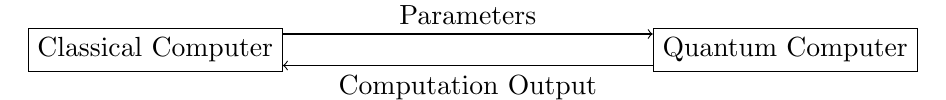
\begin{tikzpicture}[node distance = 8cm]
                \node[draw, rectangle] (C) {Classical Computer};
                \node[draw, rectangle, right of=C] (Q) {Quantum Computer};
	
                
                \begin{scope}[transform canvas={yshift=0.2cm}]
                    \draw[->] (C) -- node[above, midway] {Parameters} (Q);
                \end{scope}
                
                \begin{scope}[transform canvas={yshift=-0.2cm}]
                    \draw[->] (Q) -- node[below, midway] {Computation Output} (C);
                \end{scope}
            \end{tikzpicture}
        \end{figure}
        \vspace{1em}
    \end{center}

\end{frame}

\begin{frame}
    \frametitle{Quantum Bandaid}

    Tides us over while people look for exotic materials and configurations to
    attain reasonable coherence!

    \begin{itemize}
        \item[\textcolor{OliveGreen}{\checkmark}] Computational efficiency of a quantum computer
        \item[\textcolor{OliveGreen}{\checkmark}] Control efficiency of a classical system
        \item[\textcolor{OliveGreen}{\checkmark}] Allows alternate explorations for quantum supremacy
    \end{itemize}

\end{frame}

\begin{frame}
    \frametitle{A Solution}

    \begin{center}
        \textcolor{Periwinkle}{\large Variational Quantum Algorithms \footfullcite{cerezo2021vqa}}

        \begin{figure}
            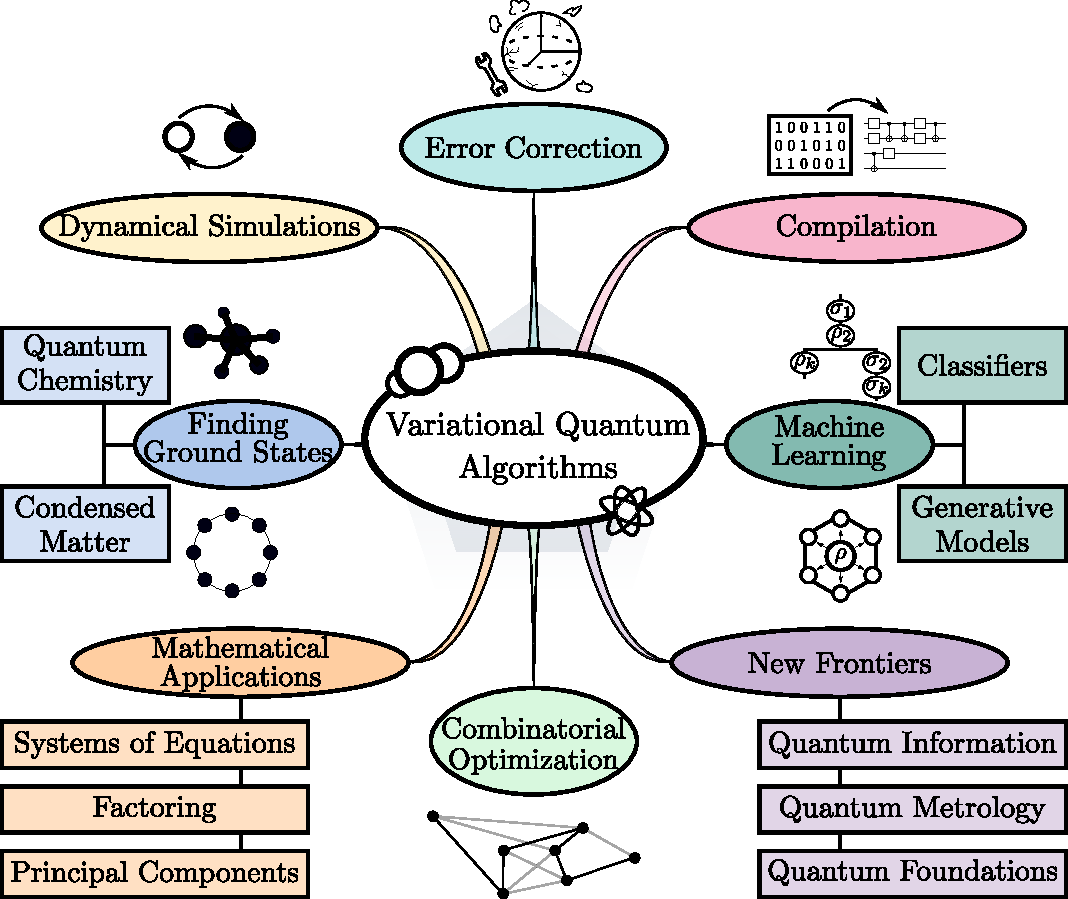
\includegraphics[width=0.4\textwidth]{figures/vqaapp.pdf}
        \end{figure}
    \end{center}

\end{frame}

    % % classification problem
    % % classical optimization is hard
    % % but nisq compatible?
    % % lead up to vqa
    % % classical.tex

% take classification as a case study
\begin{frame}
    \frametitle{(Supervised) Classification Problem}

    Given a set of input vectors with labels \({\vec{x_i}, y_i}\), learn a
    model, and attempt to predict the labels for arbitrary inputs.
    \footnote{Image: \texttt{User:ZackWeinberg} on Wikimedia Commons, CC BY-SA 3.0}

    % add diagram TODO
    \begin{figure}
        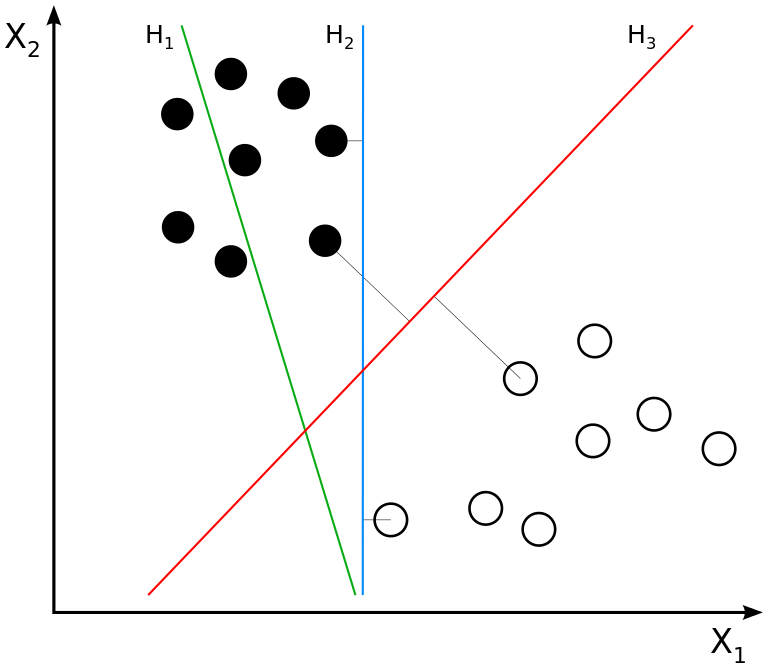
\includegraphics[width=0.4\textwidth]{figures/sephyper.png}
    \end{figure}

\end{frame}

% svm
\begin{frame}
    \frametitle{Support Vector Machines (SVM)}

    Support Vector Machine or Maximum Margin Classifier attempts to find a
    separating plane between labels and optimizes the margin, i.e., distance
    from inputs on either side to it.
    \footnote{Image: \texttt{User:Larhmam} on Wikimedia Commons, CC BY-SA 3.0}

    \begin{multicols}{2}
        % svm fig
        \begin{figure}
            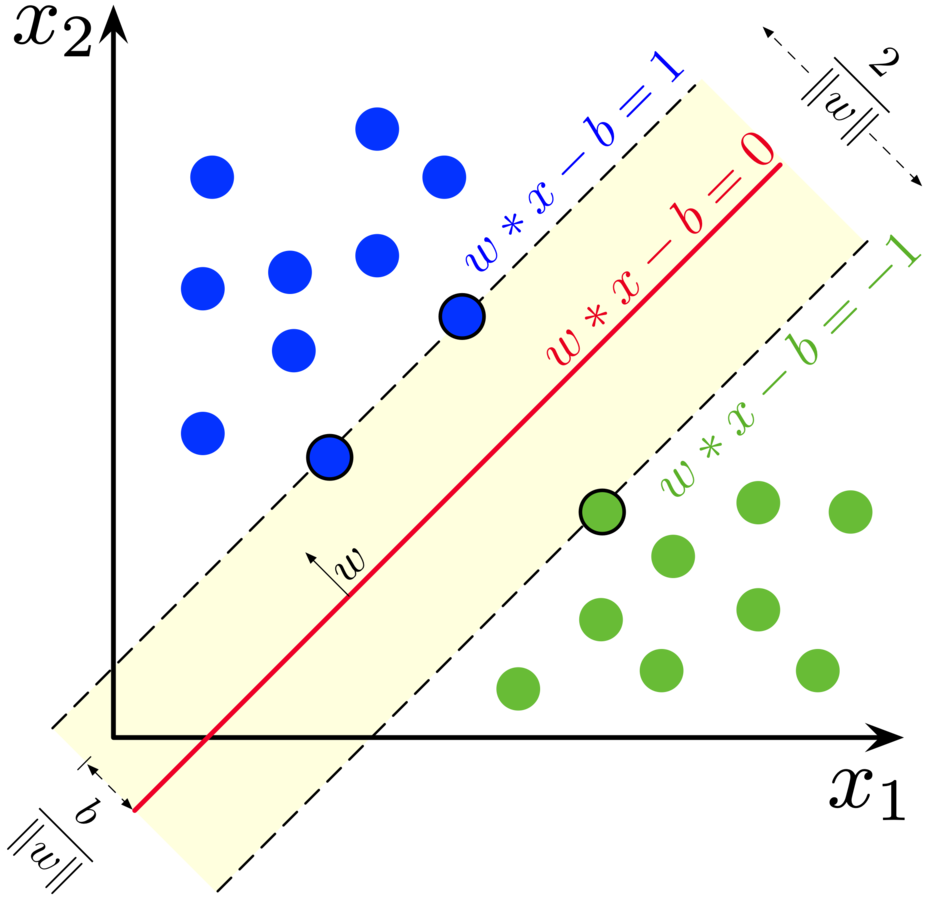
\includegraphics[width=0.4\textwidth]{figures/svmmargin.png}
        \end{figure}
        %
        Hyperplane characterized by a normal vector and a bias \((\vecw, b) \in
        \reals^{n+1}\).
        \begin{gather*}
            \innerproductabstract{\vecw}{\vec{x_i}} + b \geq 1 \text{ if } y_i = 1~, \text{and}\\
            \innerproductabstract{\vecw}{\vec{x_i}} + b \leq -1 \text{ if } y_i = -1~.
        \end{gather*}

        We minimize

        \begin{equation*}
            \mathcal{L}(\vecw, \vec{\alpha}) = \frac{1}{2} \innerprod{\vecw}{\vecw} + \sum_i \alpha_i \left[y_i \cdot \innerprod{\vecw}{\vec{x_i}}\right]~.
        \end{equation*}
    \end{multicols}

\end{frame}

% optimization is hard
\begin{frame}
    \frametitle{Optimization is hard}

    Common techniques --- gradient descent, Hessian-based descent, etc.
    %
    Lots of linear algebraic computation! 

    Matrix multiplication: \(\order{n^{2.37}}\)

    How many dimensions do we have? Consider a simple case of classifying
    \(200\times 200\) sized images, 40,000 dimensional linear algebra!

\end{frame}

% could quantum possibly help?
\begin{frame}
    \frametitle{Quantum Relief?}

    Qubits scale exponentially in the amount of information they can contain. An
    n-qubit state can carry information equivalent to \(\sim 2^n\) complex numbers!

    \begin{figure}
        \centering
        \begin{subfigure}{0.45\textwidth}
            \centering
            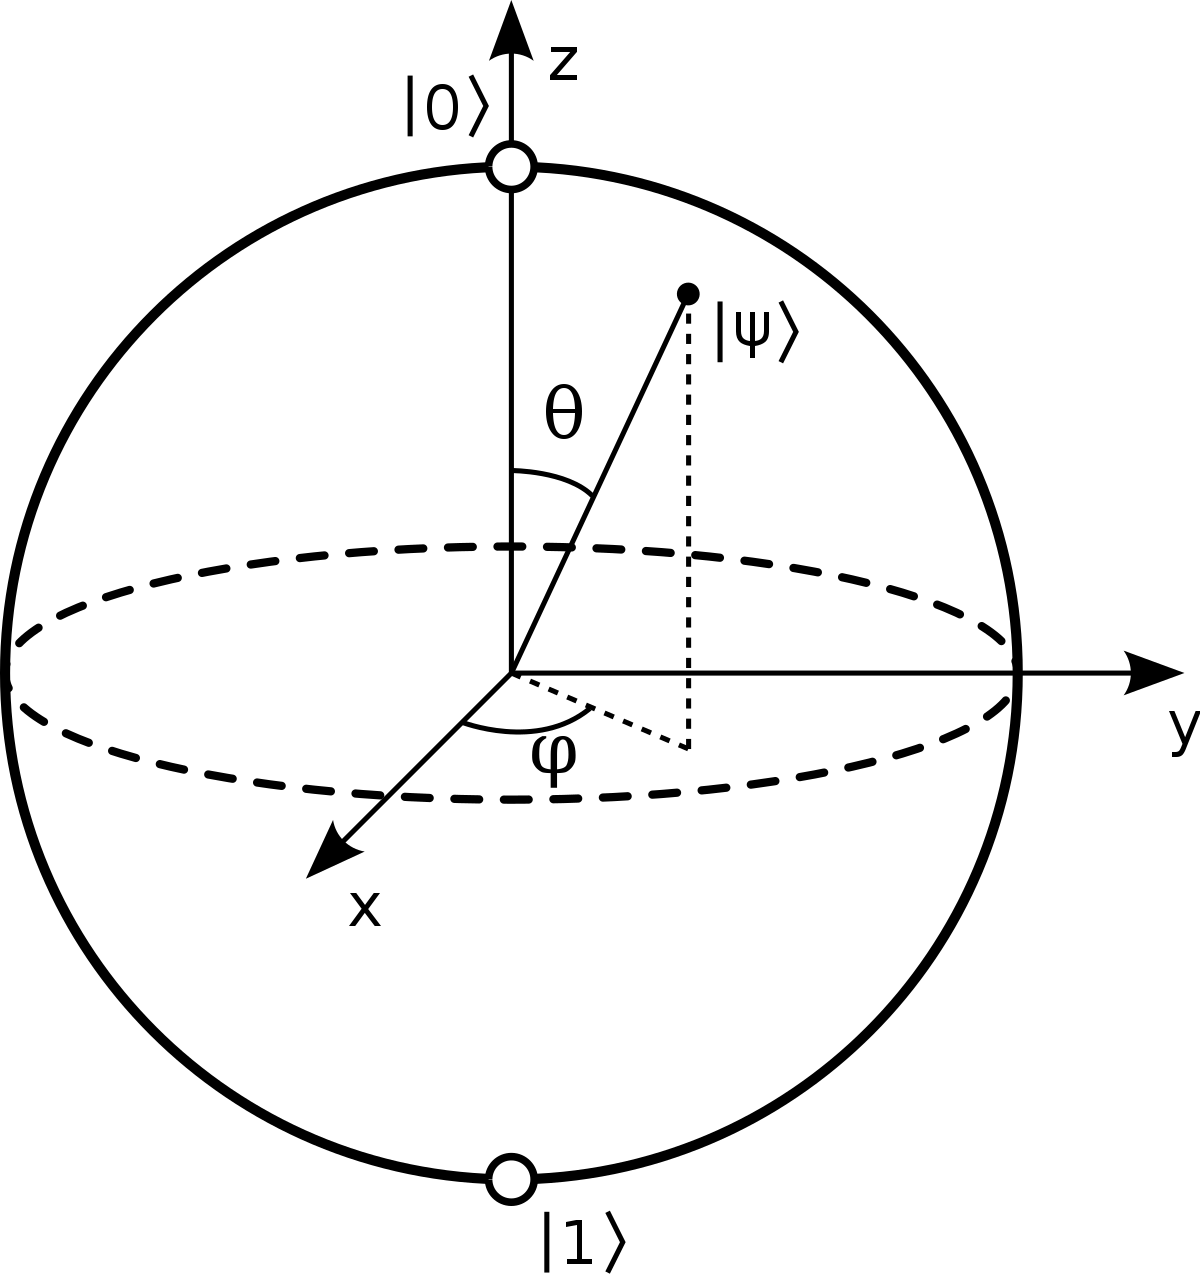
\includegraphics[width=0.5\textwidth]{figures/blochsphere.png}
        \end{subfigure}
        \begin{subfigure}{0.45\textwidth}
            \centering
            \begin{gather*}
                \begin{bmatrix}
                    c_{1,1} & c_{1,2} & \ldots & c_{1,2^n} \\
                    c_{2,1} & c_{2,2} & \ldots & c_{2,2^n} \\
                    \vdots & \ddots & \ddots & \vdots \\
                    c_{2^n,1} & c_{2^n,2} & \ldots & c_{2^n,2^n}
                \end{bmatrix}
            \end{gather*}
        \end{subfigure}
    \end{figure}

    The scale of computation is suddenly reduced. Instead of 40,000 dimension
    classical computation, we may only need \(\lceil{\log_2 (40000)}\rceil = 16\)
    qubit sized computation systems.

\end{frame}

% yes, vqas
\begin{frame}
    \frametitle{Quantum, sure, but NISQ?}

    In the near term, it seems the required number of qubits to outpace
    classical computers may not be out of reach. But can we reliably perform
    those computations on our quantum computers? Short coherence times make this
    impossible to do directly.

    Perhaps the constrained calculations can be processed as a subroutine? Yes,
    with \emph{Variational Quantum Algorithms}!

\end{frame}


    % vqa
    % components
    % pqc
    % dla
    % qlt
    \section{Variational Quantum Algorithms}
    % vqa.tex

% vqa structure


\begin{frame}
    \frametitle{Variational Quantum Algorithms}

    Variational Quantum Algorithms (VQA) form the idea of using a proposed
    architecture for generalised learning problems on NISQ systems
    \cite{bharti2021noisy}.

    \begin{figure}
        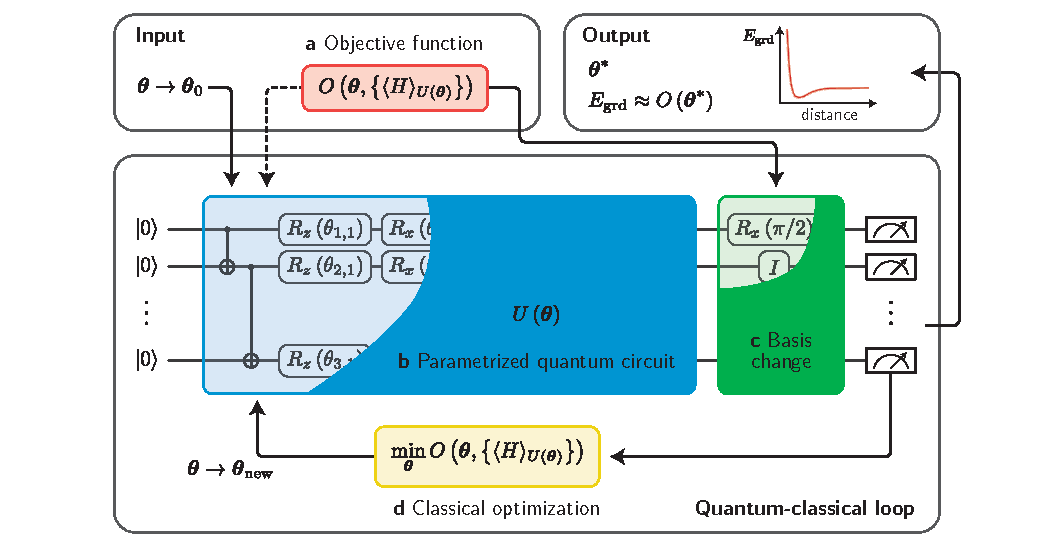
\includegraphics[width=0.8\textwidth]{figures/vqaarch.pdf}
    \end{figure}
\end{frame}

% where does this slot in?

\begin{frame}
    \frametitle{Transitioning}

    \begin{figure}
        \centering
        
        \begin{subfigure}{0.45\textwidth}
            \centering
            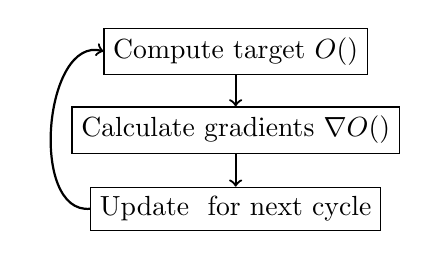
\begin{tikzpicture}[every node/.style=draw,rectangle] 
                \node (opt) [] {Compute target \(O(\vecx)\)};
                \node (grad)[below of=opt] {Calculate gradients \(\nabla O(\vecx)\)};
                \node (upd) [below of=grad] {Update \(\vecx\) for next cycle};

                \draw[->, thick] (opt) to (grad);
                \draw[->, thick] (grad) to (upd);
                \draw[->, thick, bend left=100] (upd.west) to (opt.west);
            \end{tikzpicture}
        \end{subfigure}
        %
        \pause
        \begin{subfigure}{0.45\textwidth}
            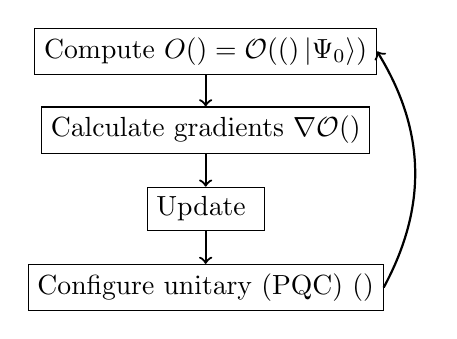
\begin{tikzpicture}[every node/.style=draw,rectangle] 
                \node (opt) [] {Compute \(O(\parameters) = \mathcal{O}(\pqc(\parameters)\ket*{\Psi_0})\)};
                \node (grad)[below of=opt] {Calculate gradients \(\nabla \mathcal{O}(\parameters)\)};
                \node (uni)[below of=grad] {Update \(\parameters\)};
                \node (upd) [below of=uni] {Configure unitary (PQC) \(\pqc(\parameters)\)};
    
                \draw[->, thick] (opt) to (grad);
                \draw[->, thick] (grad) to (uni);
                \draw[->, thick] (uni) to (upd);
                \draw[->, thick, bend right] (upd.east) to (opt.east);
            \end{tikzpicture}
        \end{subfigure}
    \end{figure}

    \begin{center}
        \(\parameters \in \reals^M, \vecx \in \reals^N, M \sim \lceil{\log_2 N}\rceil\)
    \end{center}

\end{frame}

% detailed look at PQCs
% dla
\begin{frame}
    \frametitle{Parametrized Quantum Circuits (PQCs)}

    The actual unitary computation happens in an L-layered structure with the
    mathematical form

    \begin{gather}
        \pqc(\parameters) = \prod\limits_{l = 1}^{L} U_l(\parameters_l), \quad
        \pqc_l(\parameters) = \prod\limits_{k = 1}^{K} e^{-\iota \theta_{lk} H_k}~.
        \label{eq:pqc}
    \end{gather}

    for a set of generators \(\{H_k\}\) with \(\parameters = (\parameters_1,
    \parameters_2, \ldots, \parameters_k)\).

    \pause
    Formally, the generators create a Dynamical Lie Algebra, which determines
    the set of reachable unitaries. The choice of generators can strongly affect
    the optimization process \cite{larocca2021diagnosing}. See the report for a
    detailed study.

\end{frame}

% qlt
\begin{frame}
    \frametitle{Quantum Landscape Theory}

    Spaces and maps involved in VQA calculation \cite{larocca2021theory}:

    \begin{figure}
        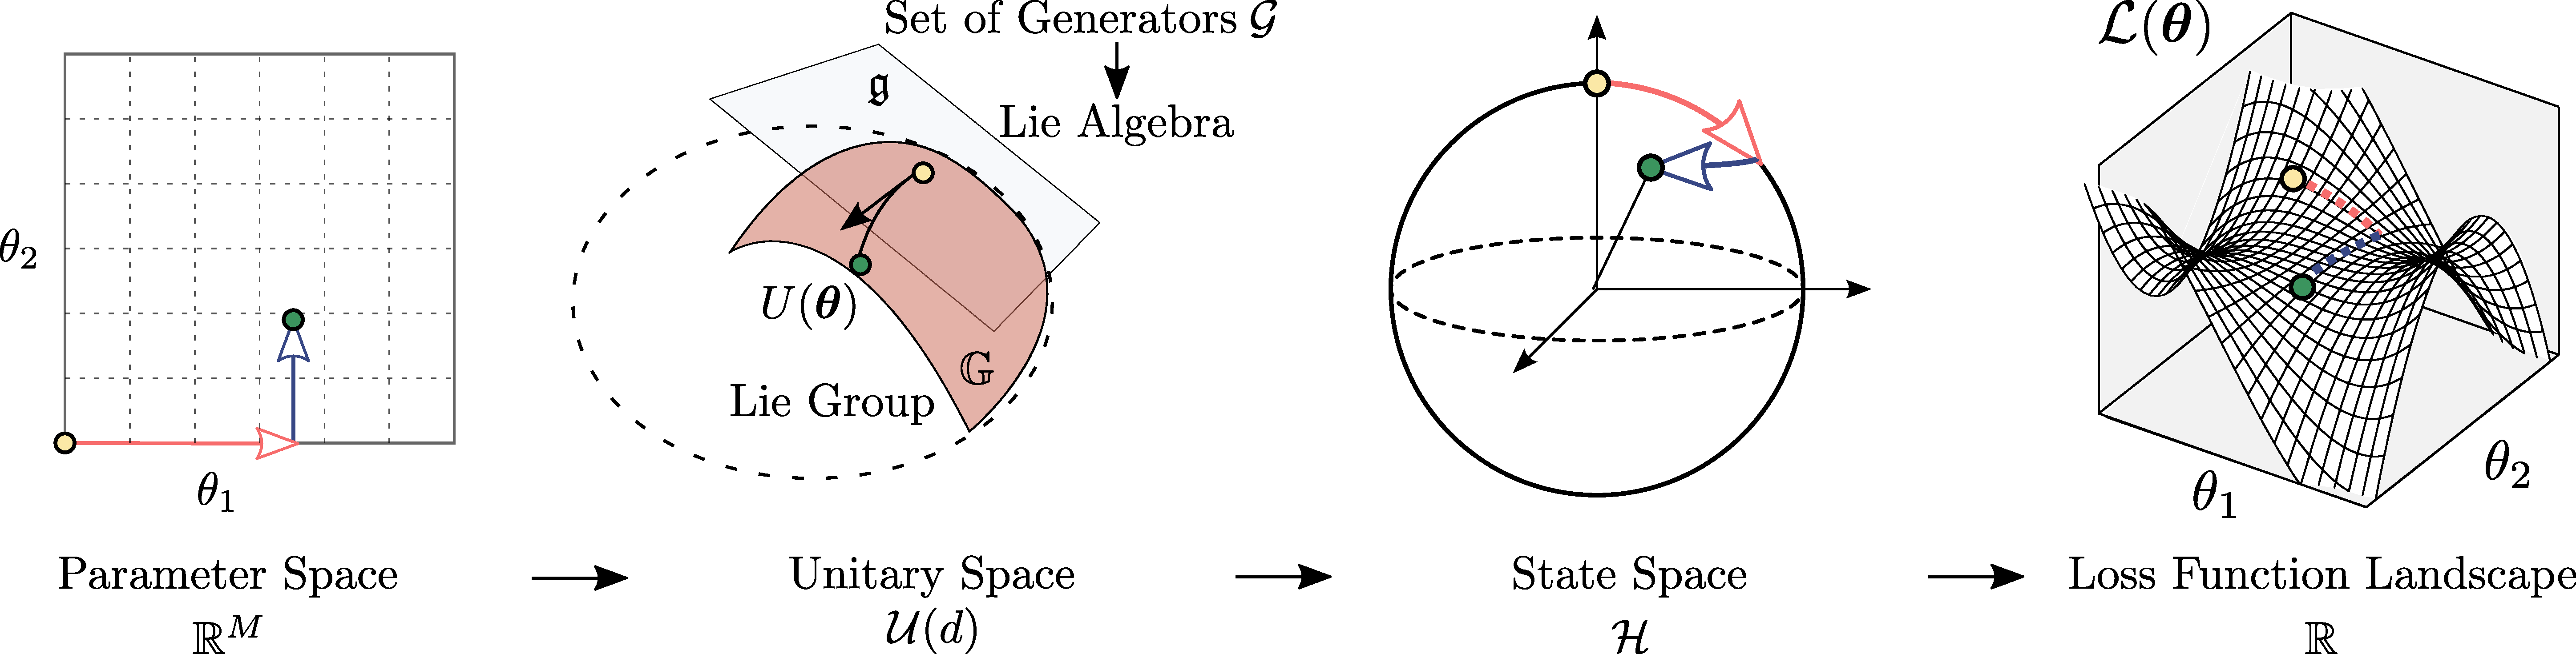
\includegraphics[width=0.8\textwidth]{figures/mapsurjective.pdf}
    \end{figure}

    This structure forms the playground for our analysis. The study of these
    spaces forms an important part of establishing relative bounds at stages of
    the calculation (which are the spaces). We discuss the particular case of
    \(\mathcal{U}(d) \to \hilbertspace\) here. See the report for details on the
    other maps.

\end{frame}


    % % info theory
    % % why limit
    % % qoc
    % % limits on svm
    % % experiments
    % % infolim.tex

% why is there a limit?
\begin{frame}
    \frametitle{Information Theoretic Limits}

    
    \begin{multicols}{2}
        
        \begin{figure}
            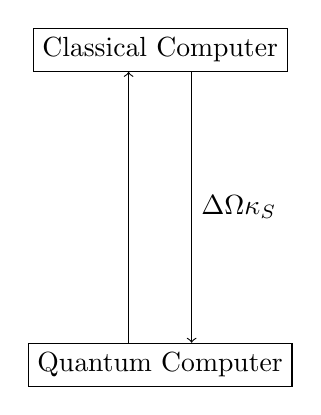
\begin{tikzpicture}[node distance = 4cm]
                \node[draw, rectangle] (C) {Classical Computer};
                \node[draw, rectangle, below of=C] (Q) {Quantum Computer};
	
                
                \begin{scope}[transform canvas={xshift=0.4cm}]
                \draw[->] (C) -- node[right, midway] {$\Delta\Omega \kappa_S$} (Q);
                \end{scope}
                
                \begin{scope}[transform canvas={xshift=-0.4cm}]
                    \draw[->] (Q) -- node[below, midway] {} (C);
                \end{scope}
            \end{tikzpicture}
        \end{figure}
        %
        The classical system transferring information about the parameters to
        the PQC has a limit on how much information it can transfer in a given
        time \(T\) given by
        \begin{gather*}
            b = T\Delta\Omega\kappa_s
        \end{gather*}
        where \(\Delta\Omega\) is the channel bandwidth and \(\kappa_s\) is the
        bit depth of the control signal (amount of information \emph{per}
        trasnfer).
    \end{multicols}

\end{frame}

% summary of bounds on qoc
\begin{frame}
    \frametitle{Example --- Bounds on Quantum Optimal Control}

    For the specific example of a control pulse for a quantum system
    \cite{lloyd2014information}

    \begin{gather*}
        \dot{\rho} = \mathcal{L}(\rho, \gamma(t))~,
    \end{gather*}

    where \(\rho\) is the state density matrix, \(\mathcal{L}\) is the
    Liouvillian operator, and \(\gamma(t)\) is the control pulse. We have the
    Hamiltonian

    \begin{gather*}
        \hamiltonian = \hamiltonian_D + \gamma(t)\cdot \hamiltonian_C~.
    \end{gather*}

\end{frame}

\begin{frame}
    \frametitle{Example --- Bounds on Quantum Optimal Control}
    
    We have

    \begin{gather*}
        \kappa_s = \log (1 + \frac{\Delta\gamma}{\delta\gamma})~,
    \end{gather*}

    where \(\Delta\gamma\) and \(\delta\gamma\) are the maximum and minimum
    variation in the control field.

    We have the error bound \footfullcite{lloyd2014information}
    \(\norm*{\rho-\rho_*} > \epsilon\), with

    \begin{gather*}
        \epsilon \geq 2^{-\frac{T\Delta\Omega\kappa_s}{\dimD_\polyreachable}}~,
    \end{gather*}

    where \(\dimD_\polyreachable\) is the dimension of the relevant
    (polynomially reachable) space of density matrices.

    \notes{We intend to employ a similar analysis to establish bounds on PQC errors.}

\end{frame}

\begin{frame}
    \frametitle{Parameter Space Dimension - Fisher Information}

    \begin{gather}
        \left[ F_\mu (\parameters)\right] = 
                4\text{Re}
                \left[
                    \braket{\partial_i \psi_\mu(\parameters)}{\partial_j \psi_\mu(\parameters)}
                % \qquad\qquad
                % \right.\nonumber\\
                % \left. \qquad\qquad
                    -
                    \braket{\partial_i \psi_\mu(\parameters)}{\psi_\mu(\parameters)}
                    \braket{\psi_\mu(\parameters)}{\partial_j \psi_\mu(\parameters)}
                \right]
    \end{gather}

    where \(\psi_\mu\) varies over the input state set.

    \(F_\mu\) is \(M\times M\) where \(M\) is the number of parameters in the
    control. \\

    \pause
    
    \begin{center}
        \emph{Increase M till rank plateaus.}
    \end{center}

    \notes{Question: What does this Mmax look like then?}

\end{frame}

\begin{frame}
    \frametitle{Parameter Scaling Bounds}

    \notes{Some suggestions have been made that polynomially growing parameter space
    anstazes can be used for VQAs. But the work is speculative and it remains to
    be seen whether any interesting problems fall within this class of 2-design
    solvability.}

    \begin{multicols}{2}
        
        \begin{center}
            \includegraphics<1>[width=0.5\textwidth]{figures/linear.pdf}
            \includegraphics<2>[width=0.5\textwidth]{figures/poly.pdf}
            \includegraphics<3>[width=0.5\textwidth]{figures/exp.pdf}
        \end{center}
        %
        \begin{itemize}
            \item<1-> Linear?
            \item<2-> Polynomial?
            \item<3-> Exponential, in general.
        \end{itemize}
    \end{multicols}

\end{frame}

\begin{frame}
    \frametitle{Trainability Tradeoff}

    What problems does this bring?
    \pause
    
    \begin{gather}
        \epsilon \geq e^{-\frac{T\Delta\Omega\kappa_S}{\dimD_{\polyreachable}}}~,\\
        T\Delta\Omega\kappa_S \geq \dimD_{\polyreachable}\ln(\frac{1}{\epsilon})~.
    \end{gather}

\end{frame}

\begin{frame}
    \frametitle{Consequences?}

    \begin{itemize}[<+->]
        \item Not a complexity bound! \footfullcite{bittel2021trainingvqa}
        \item Specification constraints!
    \end{itemize}

    \notes{While training of VQAs being NP-Hard has been discussed, quantum variational
    eigensolvers and approximate optimization algorithms have been understood to
    be heuristics, and it is generally fine if the worst case complexity is bad,
    as long as for most problems you have something nice.}

    \notes{However, this is a hardware constraint. To be able to ensure we explore the
    correct solution space, designers will have to provision higher bandwidth
    devices for all test cases, and as such we think this may have serious
    consequences for design and applicability of variational quantum algorithms. }

\end{frame}

% % bounds on qsvm
% \begin{frame}
%     \frametitle{Quantum SVM}

%     Given training data embedded as n-qubit quantum states \(\{\ket*{x_i}\}\) with
%     corresponding labels \({y_i = \pm 1}\), a QSVM implemented as a VQA attempts to learn a
%     unitary \(\pqc(\parameters)\) such that

%     \begin{equation*}
%         \text{sgn }{\bra*{0}^{\otimes n}\pqc(\parameters)^*\ket*{x_i}} = y_i \forall i~.
%     \end{equation*}

%     Setting \(\ket*{w} = \pqc(\parameters)\ket*{0}^{\otimes n}\) recovers the
%     familiar classical SVM.

% \end{frame}

% \begin{frame}
%     \frametitle{Quantum SVM --- Bounds}

%     \begin{multicols}{2}
%        \scalebox{0.55}{
%             \begin{minipage}{\textwidth}
%                 \begin{figure}
%                     % error cones
%                     \centering
%                     \begin{tikzpicture}[>=stealth']
%                         % Draw axes
%                         \draw [<->,thick] (0,5) node (yaxis) [above] {}
%                             |- (5,0) node (xaxis) [right] {};
%                         \draw [<->,thick] (0,-5) node (negyaxis) [above] {}
%                             |- (-5,0) node (negxaxis) [right] {};
%                         % classifier
%                         \draw[red, thick] (-4, -4) -- (4, 4);
%                         \draw[red, thick,->] (0, 0) -- node[very near end, right] {\(~\ket*{w}\)} (+1, -1);
%                         % error bars
%                         \draw (-3.5, -4.5) -- (3.5, 4.5) [dashed];
%                         \draw[->] (0, 0) -- (1.2, -0.8)[dashed];
%                         \draw (-4.5, -3.5) -- (4.5, 3.5) [dashed];
%                         \draw[->] (0, 0) -- node[very near end, below] {\(\ket*{w_\epsilon}\)} (0.8, -1.2)[dashed];
%                     \end{tikzpicture}
%                 \end{figure}
%             \end{minipage}
%         }

%         Picking a point randomly in the space outside the training data and
%         attempting to classify it we find \cite{li2011concise}

%         \begin{align}
%             p_{\text{error}} &= \lim_{r\to \infty}\frac{2\cdot V_{\text{sector}}(r)}{V_{\text{sphere}}(r)} \nonumber\\
%                 &= \lim_{r\to \infty}\frac{2\cdot V_{\text{sphere}}(r)\cdot 0.5\cdot I_{\text{sin}^2\phi}(\frac{n-1}{2}, \frac{1}{2})}{V_{\text{sphere}}(r)} \nonumber\\
%                 &= I_{\text{sin}^2\phi}(\frac{n-1}{2}, \frac{1}{2})~.
%         \end{align}
%     \end{multicols}

% \end{frame}

% \begin{frame}
%     \frametitle{Quantum SVM --- Bounds}
%     \begin{align}
%         p_{\text{error}}&= I_{\text{sin}^2\phi}(\frac{n-1}{2}, \frac{1}{2})~,
%     \end{align}

%     \pause

%     where \(I\) is the incomplete Beta function, 

%     \begin{equation}
%         I_x(a, b) = \frac{B(x; a, b)}{B(a, b)} = \frac{\int_0^x t^{a-1} (1-t)^{b-1} \dd t}{\int_0^1 t^{a-1} (1-t)^{b-1} \dd t}~,
%     \end{equation}

%     \pause

%     and \(\phi\) is the angular distortion, and it is seen from \(\ket*{w} =
%     \pqc(\parameters)\ket*{0}\) that \(\text{sin} \phi \sim \epsilon\). Finally,

%     \begin{align}
%         p_{\text{error}}&= I_{\epsilon^2}(\frac{n-1}{2}, \frac{1}{2})~.
%     \end{align}

% \end{frame}

% % proposed bounds on pqc
% \begin{frame}
%     \frametitle{Quantum SVM --- Bound plots}

%     \begin{figure}
%         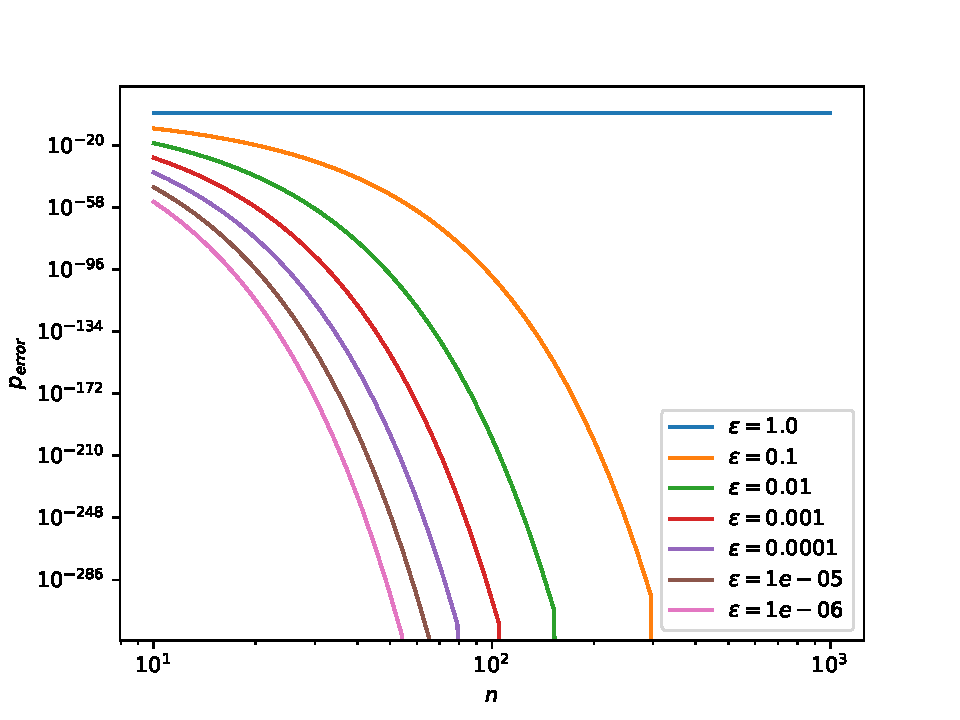
\includegraphics[width=0.8\textwidth]{figures/perrorplot.pdf}
%     \end{figure}

% \end{frame}

% \begin{frame}
%     \frametitle{Quantum SVM --- Bound plots}

%     \begin{figure}
%         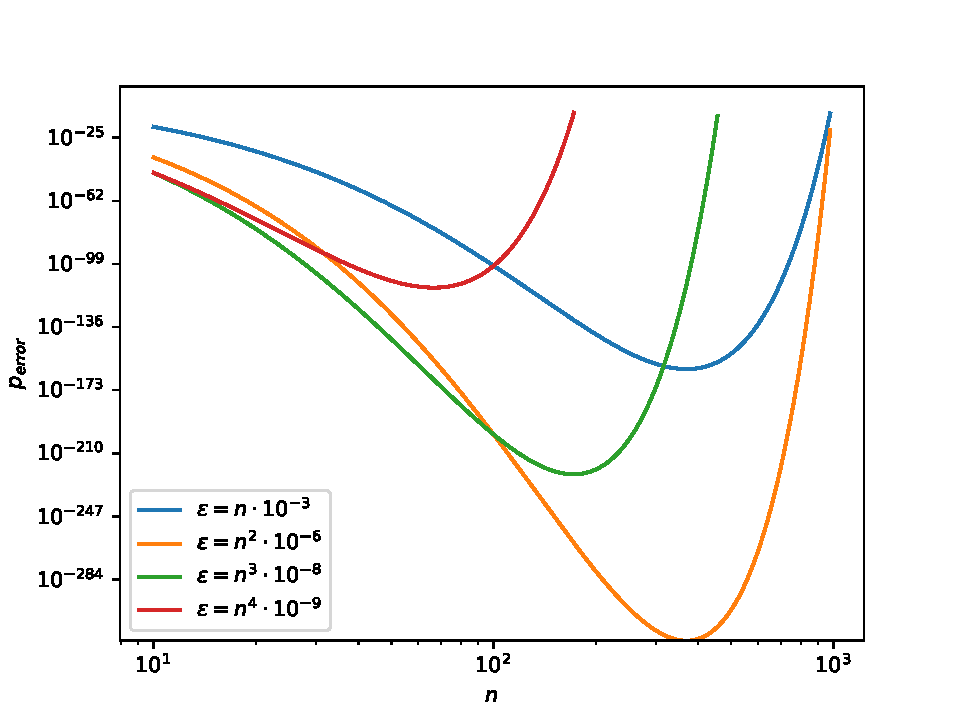
\includegraphics[width=0.8\textwidth]{figures/perrorscaled.pdf}
%     \end{figure}

% \end{frame}

    % info theory
    % why limit
    % qoc
    % ansatz expressibility
    % trainability tradeoff
    % limits of expressibility
    \section{Information Theoretic Bounds}
    % infolim.tex

% why is there a limit?
\begin{frame}
    \frametitle{Information Theoretic Limits}

    
    \begin{multicols}{2}
        
        \begin{figure}
            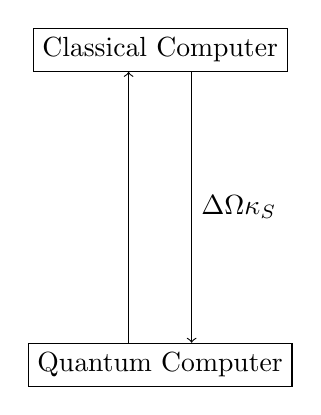
\begin{tikzpicture}[node distance = 4cm]
                \node[draw, rectangle] (C) {Classical Computer};
                \node[draw, rectangle, below of=C] (Q) {Quantum Computer};
	
                
                \begin{scope}[transform canvas={xshift=0.4cm}]
                \draw[->] (C) -- node[right, midway] {$\Delta\Omega \kappa_S$} (Q);
                \end{scope}
                
                \begin{scope}[transform canvas={xshift=-0.4cm}]
                    \draw[->] (Q) -- node[below, midway] {} (C);
                \end{scope}
            \end{tikzpicture}
        \end{figure}
        %
        The classical system transferring information about the parameters to
        the PQC has a limit on how much information it can transfer in a given
        time \(T\) given by
        \begin{gather*}
            b = T\Delta\Omega\kappa_s
        \end{gather*}
        where \(\Delta\Omega\) is the channel bandwidth and \(\kappa_s\) is the
        bit depth of the control signal (amount of information \emph{per}
        trasnfer).
    \end{multicols}

\end{frame}

% summary of bounds on qoc
\begin{frame}
    \frametitle{Example --- Bounds on Quantum Optimal Control}

    For the specific example of a control pulse for a quantum system
    \cite{lloyd2014information}

    \begin{gather*}
        \dot{\rho} = \mathcal{L}(\rho, \gamma(t))~,
    \end{gather*}

    where \(\rho\) is the state density matrix, \(\mathcal{L}\) is the
    Liouvillian operator, and \(\gamma(t)\) is the control pulse. We have the
    Hamiltonian

    \begin{gather*}
        \hamiltonian = \hamiltonian_D + \gamma(t)\cdot \hamiltonian_C~.
    \end{gather*}

\end{frame}

\begin{frame}
    \frametitle{Example --- Bounds on Quantum Optimal Control}
    
    We have

    \begin{gather*}
        \kappa_s = \log (1 + \frac{\Delta\gamma}{\delta\gamma})~,
    \end{gather*}

    where \(\Delta\gamma\) and \(\delta\gamma\) are the maximum and minimum
    variation in the control field.

    We have the error bound \footfullcite{lloyd2014information}
    \(\norm*{\rho-\rho_*} > \epsilon\), with

    \begin{gather*}
        \epsilon \geq 2^{-\frac{T\Delta\Omega\kappa_s}{\dimD_\polyreachable}}~,
    \end{gather*}

    where \(\dimD_\polyreachable\) is the dimension of the relevant
    (polynomially reachable) space of density matrices.

    \notes{We intend to employ a similar analysis to establish bounds on PQC errors.}

\end{frame}

\begin{frame}
    \frametitle{Parameter Space Dimension - Fisher Information}

    \begin{gather}
        \left[ F_\mu (\parameters)\right] = 
                4\text{Re}
                \left[
                    \braket{\partial_i \psi_\mu(\parameters)}{\partial_j \psi_\mu(\parameters)}
                % \qquad\qquad
                % \right.\nonumber\\
                % \left. \qquad\qquad
                    -
                    \braket{\partial_i \psi_\mu(\parameters)}{\psi_\mu(\parameters)}
                    \braket{\psi_\mu(\parameters)}{\partial_j \psi_\mu(\parameters)}
                \right]
    \end{gather}

    where \(\psi_\mu\) varies over the input state set.

    \(F_\mu\) is \(M\times M\) where \(M\) is the number of parameters in the
    control. \\

    \pause
    
    \begin{center}
        \emph{Increase M till rank plateaus.}
    \end{center}

    \notes{Question: What does this Mmax look like then?}

\end{frame}

\begin{frame}
    \frametitle{Parameter Scaling Bounds}

    \notes{Some suggestions have been made that polynomially growing parameter space
    anstazes can be used for VQAs. But the work is speculative and it remains to
    be seen whether any interesting problems fall within this class of 2-design
    solvability.}

    \begin{multicols}{2}
        
        \begin{center}
            \includegraphics<1>[width=0.5\textwidth]{figures/linear.pdf}
            \includegraphics<2>[width=0.5\textwidth]{figures/poly.pdf}
            \includegraphics<3>[width=0.5\textwidth]{figures/exp.pdf}
        \end{center}
        %
        \begin{itemize}
            \item<1-> Linear?
            \item<2-> Polynomial?
            \item<3-> Exponential, in general.
        \end{itemize}
    \end{multicols}

\end{frame}

\begin{frame}
    \frametitle{Trainability Tradeoff}

    What problems does this bring?
    \pause
    
    \begin{gather}
        \epsilon \geq e^{-\frac{T\Delta\Omega\kappa_S}{\dimD_{\polyreachable}}}~,\\
        T\Delta\Omega\kappa_S \geq \dimD_{\polyreachable}\ln(\frac{1}{\epsilon})~.
    \end{gather}

\end{frame}

\begin{frame}
    \frametitle{Consequences?}

    \begin{itemize}[<+->]
        \item Not a complexity bound! \footfullcite{bittel2021trainingvqa}
        \item Specification constraints!
    \end{itemize}

    \notes{While training of VQAs being NP-Hard has been discussed, quantum variational
    eigensolvers and approximate optimization algorithms have been understood to
    be heuristics, and it is generally fine if the worst case complexity is bad,
    as long as for most problems you have something nice.}

    \notes{However, this is a hardware constraint. To be able to ensure we explore the
    correct solution space, designers will have to provision higher bandwidth
    devices for all test cases, and as such we think this may have serious
    consequences for design and applicability of variational quantum algorithms. }

\end{frame}

% % bounds on qsvm
% \begin{frame}
%     \frametitle{Quantum SVM}

%     Given training data embedded as n-qubit quantum states \(\{\ket*{x_i}\}\) with
%     corresponding labels \({y_i = \pm 1}\), a QSVM implemented as a VQA attempts to learn a
%     unitary \(\pqc(\parameters)\) such that

%     \begin{equation*}
%         \text{sgn }{\bra*{0}^{\otimes n}\pqc(\parameters)^*\ket*{x_i}} = y_i \forall i~.
%     \end{equation*}

%     Setting \(\ket*{w} = \pqc(\parameters)\ket*{0}^{\otimes n}\) recovers the
%     familiar classical SVM.

% \end{frame}

% \begin{frame}
%     \frametitle{Quantum SVM --- Bounds}

%     \begin{multicols}{2}
%        \scalebox{0.55}{
%             \begin{minipage}{\textwidth}
%                 \begin{figure}
%                     % error cones
%                     \centering
%                     \begin{tikzpicture}[>=stealth']
%                         % Draw axes
%                         \draw [<->,thick] (0,5) node (yaxis) [above] {}
%                             |- (5,0) node (xaxis) [right] {};
%                         \draw [<->,thick] (0,-5) node (negyaxis) [above] {}
%                             |- (-5,0) node (negxaxis) [right] {};
%                         % classifier
%                         \draw[red, thick] (-4, -4) -- (4, 4);
%                         \draw[red, thick,->] (0, 0) -- node[very near end, right] {\(~\ket*{w}\)} (+1, -1);
%                         % error bars
%                         \draw (-3.5, -4.5) -- (3.5, 4.5) [dashed];
%                         \draw[->] (0, 0) -- (1.2, -0.8)[dashed];
%                         \draw (-4.5, -3.5) -- (4.5, 3.5) [dashed];
%                         \draw[->] (0, 0) -- node[very near end, below] {\(\ket*{w_\epsilon}\)} (0.8, -1.2)[dashed];
%                     \end{tikzpicture}
%                 \end{figure}
%             \end{minipage}
%         }

%         Picking a point randomly in the space outside the training data and
%         attempting to classify it we find \cite{li2011concise}

%         \begin{align}
%             p_{\text{error}} &= \lim_{r\to \infty}\frac{2\cdot V_{\text{sector}}(r)}{V_{\text{sphere}}(r)} \nonumber\\
%                 &= \lim_{r\to \infty}\frac{2\cdot V_{\text{sphere}}(r)\cdot 0.5\cdot I_{\text{sin}^2\phi}(\frac{n-1}{2}, \frac{1}{2})}{V_{\text{sphere}}(r)} \nonumber\\
%                 &= I_{\text{sin}^2\phi}(\frac{n-1}{2}, \frac{1}{2})~.
%         \end{align}
%     \end{multicols}

% \end{frame}

% \begin{frame}
%     \frametitle{Quantum SVM --- Bounds}
%     \begin{align}
%         p_{\text{error}}&= I_{\text{sin}^2\phi}(\frac{n-1}{2}, \frac{1}{2})~,
%     \end{align}

%     \pause

%     where \(I\) is the incomplete Beta function, 

%     \begin{equation}
%         I_x(a, b) = \frac{B(x; a, b)}{B(a, b)} = \frac{\int_0^x t^{a-1} (1-t)^{b-1} \dd t}{\int_0^1 t^{a-1} (1-t)^{b-1} \dd t}~,
%     \end{equation}

%     \pause

%     and \(\phi\) is the angular distortion, and it is seen from \(\ket*{w} =
%     \pqc(\parameters)\ket*{0}\) that \(\text{sin} \phi \sim \epsilon\). Finally,

%     \begin{align}
%         p_{\text{error}}&= I_{\epsilon^2}(\frac{n-1}{2}, \frac{1}{2})~.
%     \end{align}

% \end{frame}

% % proposed bounds on pqc
% \begin{frame}
%     \frametitle{Quantum SVM --- Bound plots}

%     \begin{figure}
%         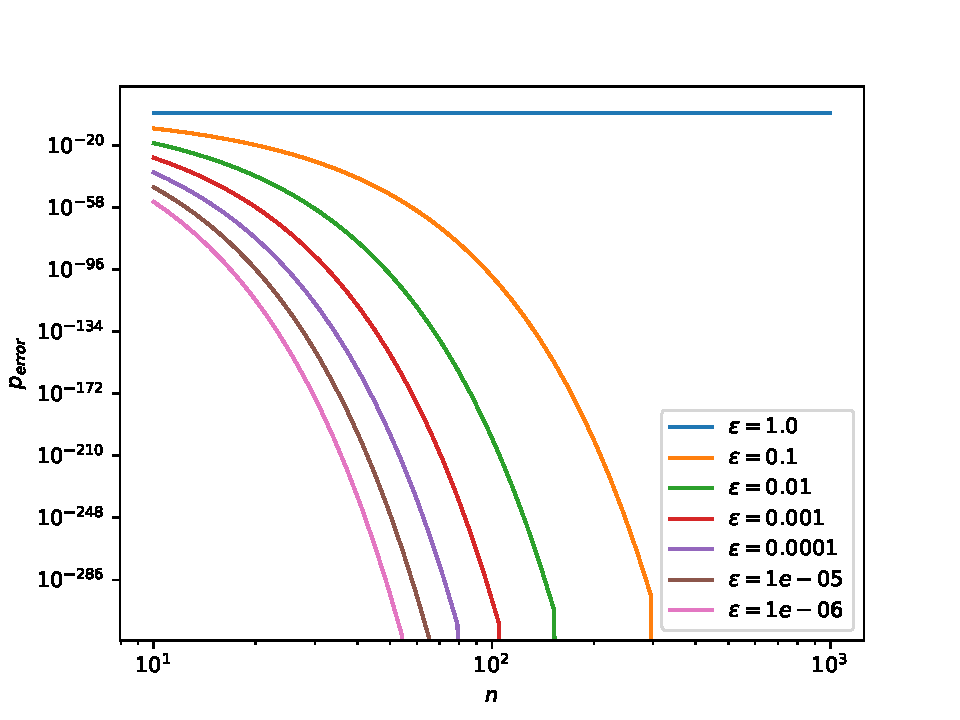
\includegraphics[width=0.8\textwidth]{figures/perrorplot.pdf}
%     \end{figure}

% \end{frame}

% \begin{frame}
%     \frametitle{Quantum SVM --- Bound plots}

%     \begin{figure}
%         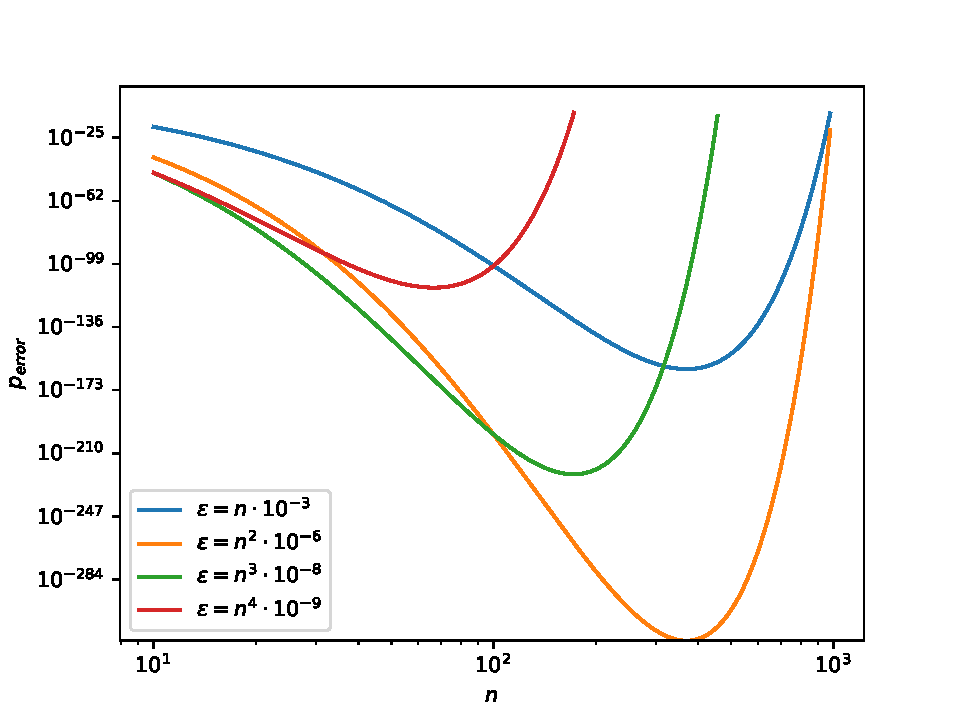
\includegraphics[width=0.8\textwidth]{figures/perrorscaled.pdf}
%     \end{figure}

% \end{frame}

    \begin{frame}{References}
        \printbibliography
    \end{frame}
\end{document}